\documentclass[10pt]{article}

\usepackage[margin=0.85in]{geometry}
\usepackage{booktabs}
\usepackage{array}
\usepackage{amsmath}
\usepackage{graphicx}
\usepackage{enumitem}
\usepackage{float} 

\title{Assignment 1}
\author{Biprarshi Biswas}
\date{\today}

\begin{document}
\maketitle

% =====================================================================
\section{Introduction}

This document is the supplementary report for Assignment 1. A frame based data transmission
system with error detection. The system establishes a TCP socket
connection between a sender and a receiver process. It builds fixed
size frames from an input file, computes a frame check sequence using
either a 16 bit checksum or one of four CRC variants, and verifies
each frame at the receiver. A separate error injection module tests
all error detection schemes against several classes of corruption to confirm their
theoretical detection guarantees. Finally, a performance module measures the
computational throughput of each scheme.

The report covers four parts. Section~\ref{sec:architecture} describes the system
architecture and file layout. Section~\ref{sec:error} explains the mathematics
behind checksum and CRC. Section~\ref{sec:error_inject} covers the error injection module
and its results. Finally, Section~\ref{sec:perf} compares computational performance of all error detection schemes discussed.

% =====================================================================
\section{Architecture}\label{sec:architecture}
This section provides an overview of the techincal architecture of the implementation. We document a tour of various modules and their respective functions.

\subsection{File Structure}

Build artifacts and log files are omitted below for readability.

\begin{verbatim}
.
|-- lab1/
|   |-- data.txt
|   |-- error.c, error.h
|   |-- frame.h
|   |-- scheme.c, scheme.h
|   |-- sender.c, receiver.c
|   |-- Makefile
|   |-- README.md
|   |-- error_inject/
|   |   |-- bit_flip.c, bit_flip.h
|   |   |-- targeted_inject.c, targeted_inject.h
|   |   `-- eval_main.c
|   |-- perf_analysis/
|   |   |-- perf_analyzer.c, perf_analyzer.h
|   |   `-- perf_main.c
|   |-- tests/
|   |   |-- error_test.c, checksum_test.c, crc_test.c
|   |   |-- scheme_test.c, boundary_test.c
|   |   `-- (additional exploratory tests)
`-- utils/
    |-- utils.c
    `-- utils.h
\end{verbatim}

\subsection{Network Utilities}

\texttt{utils.c/h} provides a scheme agnostic TCP layer used by both
sender and receiver across asignment.  Connection setup functions (listen, accept,
connect) accompanied with transfer functions that loop until a full
buffer is sent or received through \texttt{read}/\texttt{write} calls.

\subsection{Frame Structure}

Every frame is 64 bytes, split into three fixed regions.

\begin{verbatim}
[ HEADER 16B ][ PAYLOAD 44B ][ TRAILER 4B ]
\end{verbatim}

\begin{table}[htbp]
\centering
\begin{tabular}{lll}
\toprule
Field & Size & Purpose \\
\midrule
Source address & 6 B & Sender identifier \\
Destination address & 6 B & Receiver identifier \\
Frame length & 2 B & Valid payload bytes in this frame ($\leq 44$) \\
Frame sequence & 2 B & Ordering \\
Payload & 44 B & User data payload \\
FCS (trailer) & 4 B & Checksum or CRC result, zero extended \\
\bottomrule
\end{tabular}
\caption{Frame field layout}
\end{table}

The 64 byte size matches the Ethernet 802.3 minimum frame size. The
FCS is computed solely over the header and payload.

\subsection{FCS Compute and Verify}

The sender fills the header, converts host byte order to network
byte order and finally computes the FCS over the header and payload region
and stores it in the trailer. The receiver recomputes the error detection function
function over the same region and compares against the received FCS. Section~\ref{sec:error} covers the mathematics of all error schemes in detail.

\subsection{Error Injection Module}

A dedicated module (\texttt{error\_inject/}) introduces controlled
corruption into a frame after its FCS has been computed, then checks
whether checksum and CRC can detect the corruption. It includes both randomized and deliberate error injectors that target vulnerablities in error detection. Full detail and results are documented in Section~\ref{sec:error_inject}.

\subsection{Performance Analysis Module}

A separate module (\texttt{perf\_analysis/}) measures sustained
computational throughput of each scheme under a fixed time budget.
Full detail and results are in Section~\ref{sec:perf}.

\subsection{Test Suite}

Implementation of project followed test-driven-development convention, adding tests as milestones reached covering
both normal and boundary behavior.

\begin{table}[H]
\centering
\begin{tabular}{ll}
\toprule
Test File & Coverage \\
\midrule
\texttt{error\_test.c} & Integration: checksum + all CRC variants \\
\texttt{checksum\_test.c} & 10 tests: edge cases, patterns, bit flips \\
\texttt{crc\_test.c} & 8 tests: empty data, standard vectors, uniqueness \\
\texttt{scheme\_test.c} & 8 tests: dispatcher parsing, independence, tampering \\
\texttt{boundary\_test.c} & 10 tests: exhaustive Hamming distance checks \\
\bottomrule
\end{tabular}
\caption{Test coverage by file}
\end{table}

% =====================================================================
\section{Error Detection Schemes}\label{sec:error}
This section documents the mathematical reasoning behind Checksum and CRC error detection algorithms. 

\subsection{16-bit Checksum}

The message is split into 16 bit words $w_1, \dots, w_n$ and 
are added using one's complement addition. Here, ordinary binary addition is carried out,
except any carry out on bit $15$ is added back into bit $0$. This is equivalent to computing

\[
S = \left(\sum_{i=1}^{n} w_i\right) \bmod (2^{16}-1)
\]

The checksum is the bitwise complement of this sum, $C = \overline{S}$.
Complementing a value and adding it back to the original 
yields all ones: $S + C = 2^{16}-1$.

For verification, the receiver adds every received word, including the
checksum field itself, using the same one's complement addition. If
no error occurred, this sum folds to exactly $2^{16}-1$ (all ones,
\texttt{0xFFFF}). Any other result means the frame is corrupt and subsequently rejected.

The final complement step exists specifically to remove a known blind
spot. A message and checksum field that are both zeroed either deliberately or through a fault would sum to zero and pass silently, since zero is a valid sum for a naive scheme. With the complement, an all zero
message has checksum \texttt{0xFFFF} and this failure mode is addressed.

\subsection{Cyclic Redundancy Check}

A message of $n$ bits is treated as a polynomial $M(x)$ over
$\mathrm{GF}(2)$, where each bit acts as a coefficient. A generator
polynomial $G(x)$ of degree $r$ is fixed in advance. The sender
computes the remainder $R(x)$ of $M(x) \cdot x^r$ divided by $G(x)$,
using polynomial division over $\mathrm{GF}(2)$. The transmitted codeword is

\[
T(x) = M(x)\cdot x^r + R(x)
\]

which is always exactly divisible by $G(x)$.

The receiver divides the received bits by $G(x)$. A remainder of zero means no error was detected and any other
results means the frame is corrupt and subsequently rejected. In practice this division is
computed bit by bit with a shift register of width $r$: each incoming
bit shifts into the register, and whenever the bit shifted out is a
one, the register is XORed with $G(x)$.

\begin{table}[htbp]
\centering
\small
\begin{tabular*}{\textwidth}{l @{\extracolsep{\fill}} ll}
\toprule
Scheme & Generator Polynomial & Hex \\
\midrule
CRC-8  & $x^8+x^7+x^6+x^4+x^2+1$                & \texttt{0xD5} \\
CRC-10 & $x^{10}+x^9+x^5+x^4+x+1$                & \texttt{0x233} \\
CRC-16 & $x^{16}+x^{15}+x^2+1$                   & \texttt{0x8005} \\
CRC-32 & \begin{tabular}[t]{@{}l@{}}$x^{32}+x^{26}+x^{23}+x^{22}+x^{16}+x^{12}+x^{11}+x^{10}+x^8+x^7+x^5+x^4+x^2+x+1$\end{tabular} & \texttt{0x04C11DB7} \\
\bottomrule
\end{tabular*}
\caption{Generator polynomials used}
\end{table}

The CRC error detection schemes yields three guarantees. Any single bit error
is always detected, since $G(x)$ has more than one term. Any error
with an odd number of flipped bits is detected whenever $G(x)$ has
$(x+1)$ as a factor, which holds for all four polynomials above. Any
burst error confined to $r$ or fewer consecutive bits is always
detected, since such a burst cannot be a multiple of a degree $r$
polynomial. Beyond that length, a fraction $1-2^{-r}$ of random error
patterns are still caught. However, an error is invisible when its error polynomial $E(x)$ is
itself a multiple of $G(x)$, since $T(x)$ and $T(x)+E(x)$ then leave
the same remainder

% =====================================================================
\section{Error Injection Module}\label{sec:error_inject}
This section documents the various cases of corruption and compares how each error detection scheme handles them.

\subsection{Overview}

The module has two layers in its implementation. \texttt{bit\_flip.c} provides the
primitive of flipping one specific bit in a buffer by XOR, addressed by
a global bit index. \texttt{targeted\_inject.c} builds two
vulnerablities on top of this primitive, each
aimed at one scheme's specific blind spot. \texttt{eval\_main.c} drives all test cases across trials,
logs results to console and to \texttt{results.csv}.

\subsection{Test Cases}

\begin{enumerate}[label=\arabic*)]
\setcounter{enumi}{-1}
\item \textbf{All-zero blind spot (checksum)} - where data and checksum
fields are both zeroed, checking whether the one's complement design avoids
the classic naive-sum failure mode.
\item \textbf{Compensating error (checksum)} - where the same bit column
flipped in two 16-bit words, targeting checksum's blind spot for
compensating errors that cancel each other in the sum.
\item \textbf{Generator multiple (CRC)} - where the generator polynomial's
own bit pattern is XORed into the frame.
\item \textbf{Burst length at $r$ vs $r+1$ (CRC)} - which tests the burst errors of
length $r+1$ which are caught with probability $1-2^{-r}$.
\end{enumerate}

\subsection{Results}

\begin{table}[htbp]
\centering
\begin{tabular}{lcc}
\toprule
Case & Expected & Observed \\
\midrule
0: All-zero blind spot & Undetected & Detected \\
\bottomrule
\end{tabular}
\caption{Case 0 result (single deterministic construction)}
\end{table}

\begin{table}[htbp]
\centering
\begin{tabular}{lcc}
\toprule
CRC Degree & Checksum Caught & CRC Caught \\
\midrule
8  & 0/10000 (0\%)   & 10000/10000 (100\%) \\
10 & 0/10000 (0\%)   & 10000/10000 (100\%) \\
16 & 0/10000 (0\%)   & 10000/10000 (100\%) \\
32 & 0/10000 (0\%)   & 10000/10000 (100\%) \\
\bottomrule
\end{tabular}
\caption{Case 1: compensating error, 10000 trials per degree}
\end{table}

The results above confirm our hypothesis. Checksum detection is exactly 0\% at every degree, while CRC
detects every case, since polynomial division treats the two flips as
independent bit positions rather than as a linear sum.

\begin{table}[H]
\centering
\begin{tabular}{lcc}
\toprule
CRC Degree & Checksum Caught & CRC Caught \\
\midrule
8  & 10000/10000 (100\%) & 0/10000 (0\%) \\
10 & 10000/10000 (100\%) & 0/10000 (0\%) \\
16 & 10000/10000 (100\%) & 0/10000 (0\%) \\
32 & 10000/10000 (100\%) & 0/10000 (0\%) \\
\bottomrule
\end{tabular}
\caption{Case 2: generator multiple error, 10000 trials per degree}
\end{table}

The injected pattern is exactly the generator polynomial's bits, so the corrupted codeword
remains a multiple of $G(x)$ and CRC's remainder stays zero regardless
of the underlying correuption. The same bit pattern changes the checksum's
arithmetic sum in essentially every case, so checksum detects it
every time. Results confirm out hypothesis over all four degrees.

\begin{table}[H]
\centering
\begin{tabular}{lccc}
\toprule
CRC Degree & Burst=$r$ & Burst=$r{+}1$ observed & Burst=$r{+}1$ theoretical \\
\midrule
8  & 10000/10000 & 10000/10000 (100\%) & 99.609\% \\
10 & 10000/10000 & 10000/10000 (100\%) & 99.902\% \\
16 & 10000/10000 & 10000/10000 (100\%) & 99.998\% \\
32 & 10000/10000 & 10000/10000 (100\%) & 100.000\% \\
\bottomrule
\end{tabular}
\caption{Case 3: burst error boundary, 10000 trials per degree}
\end{table}

Burst length $r$ is detected without exception at every degree, which
matches the guarantee directly. Burst length $r+1$ shows 100\%
detection at every degree as well, including CRC-8, where theory predicts a
minute miss rate.

% =====================================================================
\section{Performance Analysis}\label{sec:perf}
This section formalizes the performance metrics and compares throughput accros error detection schemes.

\subsection{Methodology}

Each scheme is run in a loop over randomly generated 64 byte
frames for a fixed 10 second window, timed with
\texttt{clock\_gettime(CLOCK\_MONOTONIC)}. The loop measures only the
FCS computation itself, with no socket I/O or frame packing included,
so the result reflects the isolated cost of the error detection algorithm. Throughput in bits per second is the primary metric.

\subsection{Results}

\begin{table}[H]
\centering
\begin{tabular}{lccc}
\toprule
Scheme & Throughput (Mbps) & Frames/sec & Speedup vs CRC-32 \\
\midrule
checksum & 1605 & 3{,}135{,}052 & 8.0$\times$ \\
crc8     & 220  & 430{,}355    & 1.1$\times$ \\
crc10    & 216  & 422{,}563    & 1.08$\times$ \\
crc16    & 203  & 396{,}787    & 1.01$\times$ \\
crc32    & 200  & 391{,}562    & 1.0$\times$ \\
\bottomrule
\end{tabular}
\caption{Sustained throughput per scheme}
\end{table}

\begin{center}
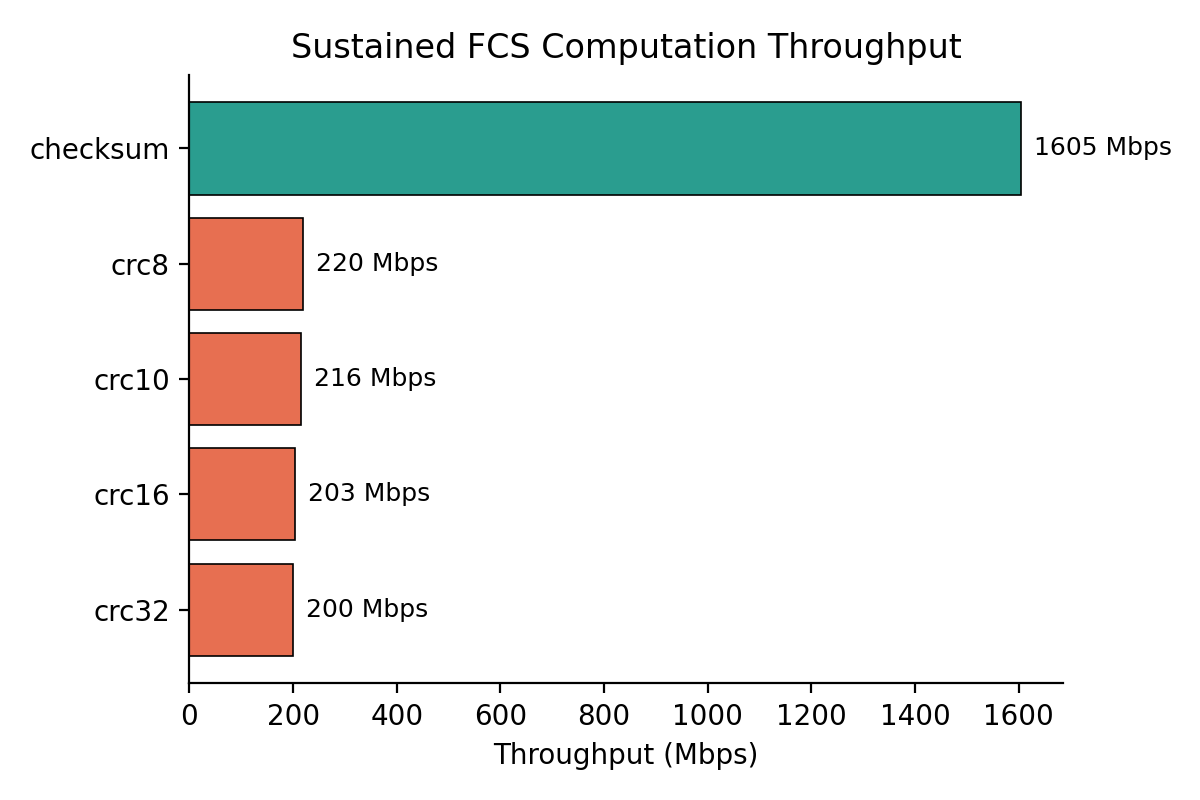
\includegraphics[width=0.58\textwidth]{perf_v2_horizontal.png}
\end{center}

\subsection{Discussion}

Checksum is roughly eight times faster than any CRC variant. Checksum
computes one addition per 16 bit word, while CRC performs a shift and
conditional XOR for every bit of input.

CRC-8 through CRC-32 cluster within about 10\% of each other despite
an eight to sixteen fold difference in output width. This is expected
under a bit serial implementation, where cost scales with the number
of input bits processed, not the register width. Therefore, widening the
polynomial from 8 to 32 bits adds fixed extra computation rather than multiplying the total cost.

Neither scheme is a practical bottleneck at typical network speeds.

\begin{center}
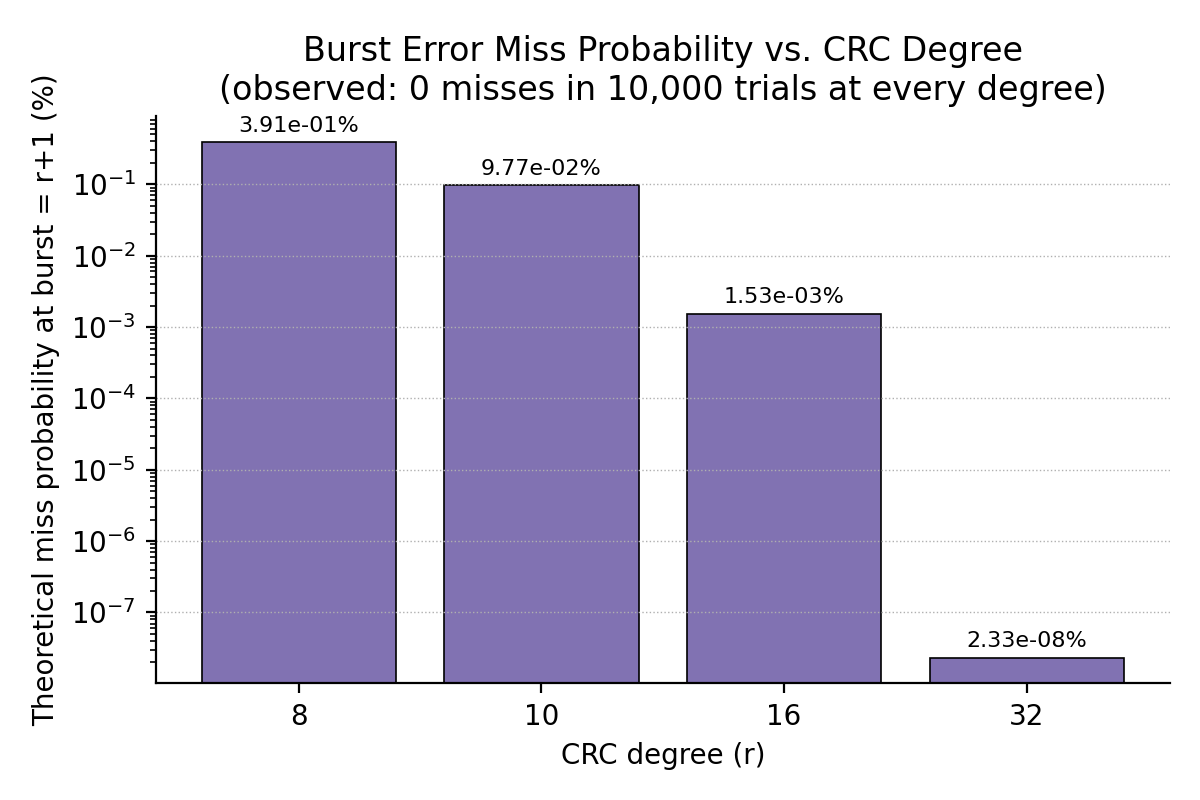
\includegraphics[width=0.58\textwidth]{burst_v2_bar.png}
\end{center}

The theoretical miss probability at burst length $r+1$ falls by
roughly two orders of magnitude for every doubling of CRC degree. This
is the reasoning behind choosing a wider polynomial when burst
errors longer than the guarantee threshold are a real possibility, at
the cost of the throughput difference discuessed above.

\end{document}